\documentclass[12pt,a4paper,ngerman,captions=tableheading]{scrartcl}

% -----------------------------------------------
% --------PAKETE-LADEN---------------------------
% -----------------------------------------------

\usepackage{acronym}

% -----------------------------------------------
% --------Seitengeometrie------------------------
% -----------------------------------------------

\usepackage{geometry}
\geometry{a4paper, top=27mm, left=30mm, right=20mm, bottom=35mm, headsep=10mm, footskip=12mm}

% -----------------------------------------------
% --------Schrift-+-Wörterbuch-------------------
% -----------------------------------------------

\usepackage[T1]{fontenc}
\usepackage[utf8]{inputenc}
\usepackage{babel}
\usepackage{lmodern}

\usepackage{microtype}
    % \setlength{\emergencystretch}{1em}

\usepackage[scaled]{helvet}
    % Serifenfreie Schrift: 
    % \renewcommand{\familydefault}{\sfdefault}

    % Zeilenabsatz - Einrücken verhindern:
\setlength{\parindent}{0em} 

    % Zeilenabstand auf 1,5: 
\usepackage[onehalfspacing]{setspace}


%------------------------------------------------------
%-----KOPF-und-FUSSZEILEN------------------------------
%------------------------------------------------------

\usepackage{scrlayer-scrpage}
%\usepackage[headtopline,headsepline]{scrlayer-scrpage}
%\setheadtopline{0,4pt}
%\setheadsepline{}

\clearscrheadfoot
\ihead{ Spezielle Messtechnik (MST2) }
\chead{Schertest}
\ohead{\today}
\ifoot*{}
\ofoot{\pagemark}
\pagestyle{scrheadings}
\setkomafont{pageheadfoot}{\small}
\setkomafont{pagehead}{}
\usepackage{breakurl}


%------------------------------------------------------
%--------Physik und Mathe------------------------------
%------------------------------------------------------

\usepackage{upgreek}

\usepackage{chemformula}
\usepackage[version=4,arrows=pgf-filled]{mhchem}

\usepackage{chemmacros} 
    \chemsetup{modules=all}

\usepackage{mathtools} % lädt auch amsmath

\usepackage{amssymb}
    % & vor entsprechendem Zeichen richtet nachfolgende Formeln daran aus
    % Leerzeilen beenden den Modus! 

\usepackage{siunitx}
\sisetup{inter-unit-product = \cdot}
\sisetup{detect-family}

    % detect-weight, % Schrifttyp übernehmen (bold, kursiv etc) 
    % detect-family, %Schriftart des Umgebungstextes übernehmen (mit/ohne Serifen) 
\DeclareUnicodeCharacter{2212}{-}

% -----------------------------------------
% ---------Links--------------------------------
% -----------------------------------------

\usepackage{url}
\urlstyle{same}



% -----------------------------------------
% -------Listen --------------------------------
% -----------------------------------------

\usepackage{mdwlist}
\usepackage{paralist}

% -------------------------------------------------------------
% Tabellen und Grafiken--------------------------------
% -------------------------------------------------------------
\usepackage{makecell}
\usepackage{graphicx}
\usepackage[lofdepth,lotdepth]{subfig}
%\usepackage{subfigure}
\usepackage{pdfpages}
\usepackage{float}
\usepackage{pdflscape}
\usepackage{tabularx}
\newcolumntype{L}[1]{>{\raggedright\arraybackslash}m{#1}} % linksbündig mit Breitenangabe
\newcolumntype{C}[1]{>{\centering\arraybackslash}m{#1}} % zentriert mit Breitenangabe
\newcolumntype{R}[1]{>{\raggedleft\arraybackslash}m{#1}} % rechtsbündig mit Breitenangabe

\usepackage{multirow}
\usepackage{array}
\usepackage{colortbl}
\definecolor{MKHgreen}{RGB}{65, 160, 55}
\usepackage{tikz}
\usetikzlibrary{external}
%\tikzexternalize
\usepackage{adjustbox}
\usepackage{pgfplots}
\usepgfplotslibrary{colorbrewer}
\pgfplotsset{compat = newest} 
% Tikz is loaded automatically by pgfplots
\usetikzlibrary{pgfplots.statistics, pgfplots.colorbrewer} 
% provides \pgfplotstabletranspose
\usepackage{pgfplotstable}
\usepackage{filecontents}

\usepackage{framed}
\usepackage{xcolor}
\colorlet{shadecolor}{gray!25}
    %\begin{shaded}
    %\end{shaded}



    %Bildunterschriften // justification=raggedright längere Bildunterschriften/Tabellenüberschriften werden linksbündig ausgerichtet, singlelinecheck=false auch kurze Bildunterschriften/Tabellenüberschriften werden linksbündig ausgerichtet
    
\usepackage{caption}
\usepackage{subcaption}
%\usepackage[labelfont=bf,font={small,sf},justification=raggedright,singlelinecheck=false]{caption} 
\addto\captionsngerman{\renewcommand{\figurename}{Abb.}}
\addto\captionsngerman{\renewcommand{\tablename}{Tab.}}


%------------------------------------------------------
%-----HYPERREF-----------------------------------------
%------------------------------------------------------

\usepackage[
  colorlinks, 
  backref=true, 
  pdfpagelabels, 
  pdfstartview=FitH, 
  bookmarksopen=true, 
  bookmarksnumbered=true, 
  pdftitle={Berichte}, 
  pdfauthor={Ahmed EN-NOUR}, 
  pdfsubject={MST}, 
  pdfcreator={}, 
  pdfproducer={}, 
  pdfkeywords={MST, Messung, Labor}, 
  pdfnewwindow=true, 
  linkcolor=black, 
  plainpages=false, 
  hypertexnames=false, 
  citecolor=black, 
  filecolor=black, 
  urlcolor=black
]{hyperref}


    % Links auf Gleitumgebungen springen nicht zur Beschriftung, sondern zum Anfang der Gleitumgebung:

\usepackage[figure,table]{hypcap}

    % \usepackage[table]{hypcap}
    % oder  
    % \usepackage[tabularx]{hypcap}
    

\usepackage[labelfont=bf,justification=RaggedRight,textfont=it]{caption}
\DeclareCaptionLabelSeparator{period-newline}{. \newline}

%------------------------------------------------------
%-----LITERATURQUELLEN---------------------------------
%------------------------------------------------------

\usepackage[babel, german=quotes]{csquotes}
\usepackage[
backend=biber,
style=alphabetic,
sorting=ynt
]{biblatex}
%\addbibresource{mybibliography.bib}
\setlength{\parindent}{0pt}

\usepackage{wrapfig}
\graphicspath{{./images/}}
\bibliography{Einzelnachweise}
    % Passt die Schriftgröße  im Quellenverzeichnis an die Normale Schriftgröße an:
\renewcommand*{\bibfont}{\normalfont}


\sisetup{output-decimal-marker = {,}}
\pgfkeys{/pgf/number format/use comma}


%------------------------------------------------------
%-----NUMMERIERUNG-------------------------------------
%------------------------------------------------------

\setcounter{secnumdepth}{3}
\usepackage{multirow}
%------------------------------------------------------
%-----WORTTRENNUNG-------------------------------------
%------------------------------------------------------

\usepackage{pgfplots}
\pgfplotsset{width=10cm,compat=1.9,every mark/.append style={solid},}
%\pgfplotsset{every mark/.append style={solid},}


% We will externalize the figures
\usepgfplotslibrary{external}

\hyphenation{Tren-nungs-kor-rek-tur}

\begin{filecontents*}{data.csv}
    Sintern,Laminiert
    62.47, 86.81, 79.48, 72.66, 96.21, 67.83, 73.42, 67.10, 0
    36.87, 27.74, 27.09, 24.46, 26.97, 24.23, 27.82, 24.83, 33.19
    \end{filecontents*}
%\usepackage[Labor=true,backref=true]{hyperref}
%------------------------------------------------------
%------------------DOKUMENT----------------------------
%------------------------------------------------------

\begin{document}

%------------------------------------------------------
%------------------Titelseite--------------------------
%------------------------------------------------------

\begin{titlepage}
\centering
\begin{onehalfspace}
    \huge \textbf{}  
    \linebreak \large \textbf{}
\end{onehalfspace}

%------------------------------------------------------
%------------------------Logo--------------------------
%------------------------------------------------------


\includegraphics[height=70pt]{Bilder/fhkiel_logo.jpg}

\vspace{0.6cm}

\begin{onehalfspace}
    \huge \textbf{Spezielle Messtechnik (MST2) – Labor}  \linebreak \large \textbf{}
\end{onehalfspace}

\vspace{0.3cm}

\begin{onehalfspace}
    \Large \textbf{Laborversuch V1:  Schertest}
\end{onehalfspace}

\vspace{1cm}
{\large Teilnehmer:} 
%{\large vorgelegt von:}
    \vspace{0.5cm}

    \begin{tabular}{l l}
        \large\textbf{Alaa Albasha}, & \textbf{Matr. Nr.: 943167} \\
        \large\textbf{Jan-Manuel Megerle}, & \textbf{Matr. Nr.: 942883} \\
        \large\textbf{Nathan Kirori}, & \textbf{Matr. Nr.: 941689} \\
        \large\textbf{Ahmed EN-NOUR}, & \textbf{Matr. Nr.: 937048} \\
    \end{tabular}


    

    \vspace{0.5cm}
    
\large \textbf{MST2\_M2 - Team 1}

\vspace{1cm}
{\large Professor:}

    \vspace{0.2cm}
    
\large \textbf{Prof. Dr.-Ing. Aylin Bicakci }

    \vspace{0.3cm}

\large \textbf{Fachhochschule Kiel \linebreak Sommersemester 2025\\}
{\large Informatik und Elektrotechnik}

\vfill
%\begin{center}
 %       28.10.2023
%\end{center}
\end{titlepage}


\newpage

%------------------------------------------------------
%------------------INHALTSVERZEICHNIS------------------
%------------------------------------------------------

\tableofcontents  
%\textbf{Anhang}
\newpage

%------------------------------------------------------
%------------------INHALT----------------------------
%------------------------------------------------------

\section{Einleitung}
Ziel:\\
Oft werden für verschiedene Materialien Bindemittel verwendet, um sie zusammenzuhalten. 
Allerdings ist es erforderlich, diese Bindemittel zu testen. 
Dazu wird ein Schertest angewendet mithilfe von zwei Prüfkörpern mit jeweils zehn Scherkörpern auf deren Bodenplatten.
Aus den Daten werden Brucharten erkannt und analysiert, und daraus wird ein Boxplot-Diagramm erstellt.


%------------------------------------------------------
%######################################################
%------------------------------------------------------

\section{Theoretische Grundlagen}
Der Schertest ist ein Verfahren zur Untersuchung der mechanischen Festigkeit von Verbindungen zwischen unterschiedlichen Materialien.  Er kommt besonders dann zum Einsatz, wenn die Belastbarkeit von Bindemitteln bewertet werden soll, die beispielsweise Metall- oder Kunststoffkomponenten miteinander verbinden.\\

Bei der Durchführung eines Schertests werden Prüfkörper, bestehend aus mehreren Scherkörpern, auf einer Bodenplatte befestigt. Mithilfe eines Schermeißels wird eine seitlich wirkende Kraft aufgebracht, die die Scherkörper kontrolliert abschert. Dabei wird sowohl die aufgewendete Kraft als auch der Weg des Meißels aufgezeichnet, um daraus ein Kraft-Weg-Diagramm zu erstellen.\\

Die zentrale Messgröße ist die mittlere Haftfestigkeit, die durch Umrechnung der gemessenen Kraft auf die Querschnittsfläche der Scherkörper N/mm² bestimmt wird.  \\

Zur statistischen Auswertung der Ergebnisse wird ein Boxplot-Diagramm erstellt. Dieses zeigt nicht nur die Verteilung der ermittelten Haftfestigkeiten, sondern erlaubt auch den direkten Vergleich verschiedener Prüfkörper. Daraus können im Endeffekt Brucharten verglichen werden, um die Art des Versagens genauer zu klassifizieren etwa als adhäsiv, kohäsiv oder gemischt.\\
Die Prüfkörper werden auf Widerstand untersucht, dieser Widerstand sagt uns wie viel Schubspannung ein Scherkörper aufnehmen kann bis Scherabriss sich bildet.\\
Es gilt folgende Formel zur Berechnung der Schubspannung:\\
\begin{equation}
    \tau = \frac{F}{A}
\end{equation}   
\vspace{0.2cm}
\begin{figure}
    \centering
    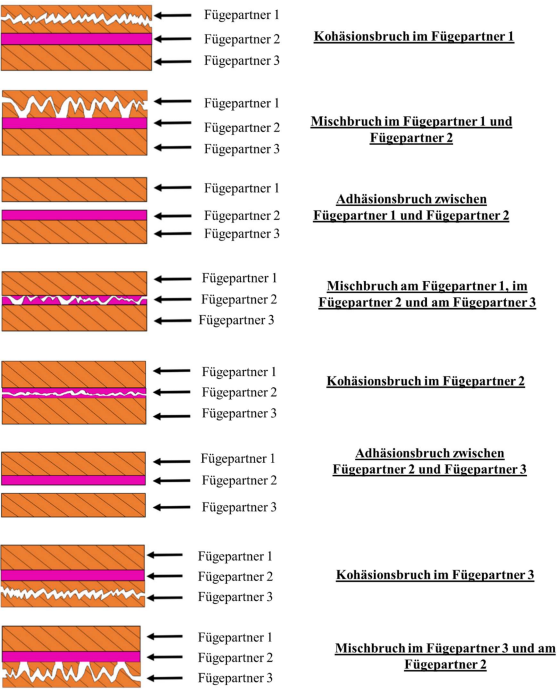
\includegraphics{Bilder/Brucharten.png}
    \caption{Mögliche Bruchbilder eines Schertests}
    \caption*{\textit{Quelle: https://tinyurl.com/2p8ejcnv }}
    \vspace{0.2cm}
    \label{Abb.3: Mögliche Bruchbilder eines Schertests}
\end{figure}
\\


%------------------------------------------------------
%######################################################
%------------------------------------------------------

%\newpage
\section{Aufgabenstellung}
Ziel dieses Versuchs ist es, die mechanischen Eigenschaften von Kupfer-Scherkörpern zu
untersuchen und zu vergleichen:\\
\subsection{Untersuchung der Prüfkörper:}
Hiermit werden zwei Kupfer-Scherkörpern untersucht mit jeweils eine Art:\\
Scherprüfling 1: Versilberter Kupfer Scherkörper gesintert auf Kupferbodenplatte.\\
\vspace{0.05cm}
\begin{figure}[h]
    \centering
    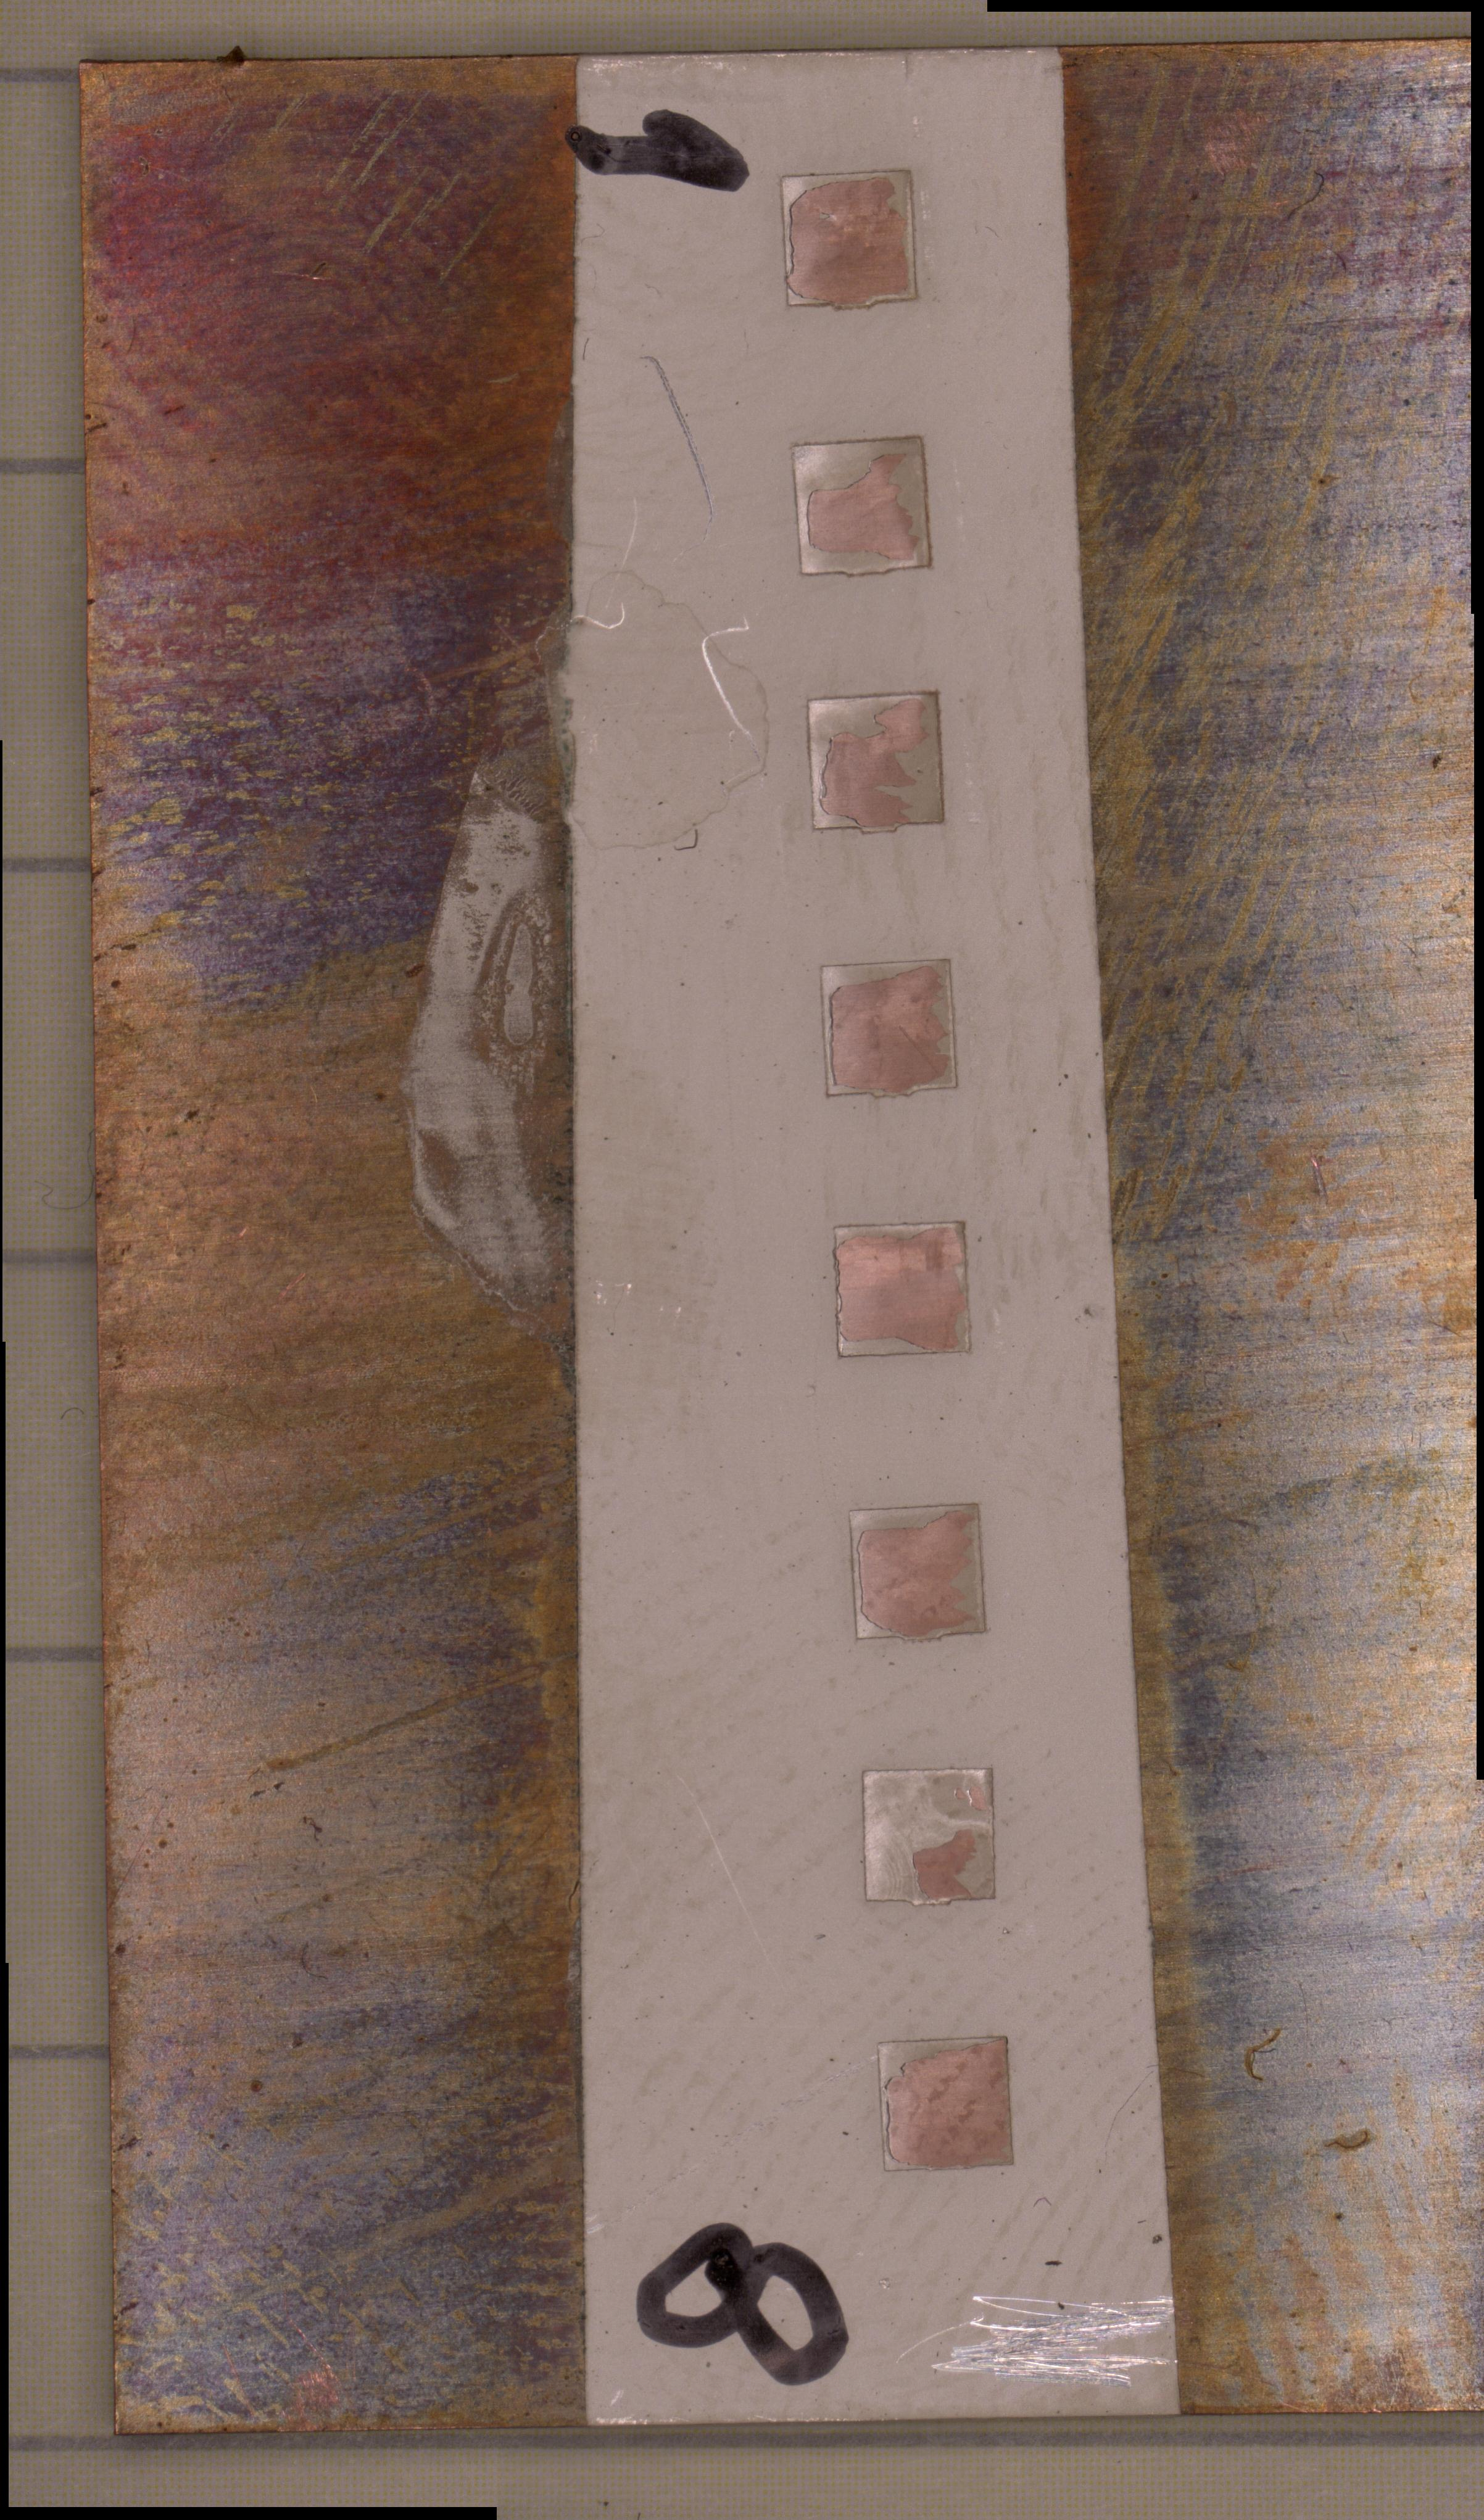
\includegraphics[scale=0.1, angle=90]{Bilder/Bodenplatte_Sintern_Gesamt.jpg}
    \caption{Versilberter Kupfer Scherkörper gesintert auf Kupferbodenplatte}
    \caption*{\textit{Quelle: Selbsterstellt}}
    \vspace{0.2cm}
    \label{Abb.2: Versilberter Kupfer Scherkörper gesintert auf Kupferbodenplatte} 
\end{figure}\\
Scherprüfling 2: Kupfer Scherkörper laminiert auf Kupferbodenplatte
\vspace{0.1cm}
\begin{figure}[h]
    \centering
    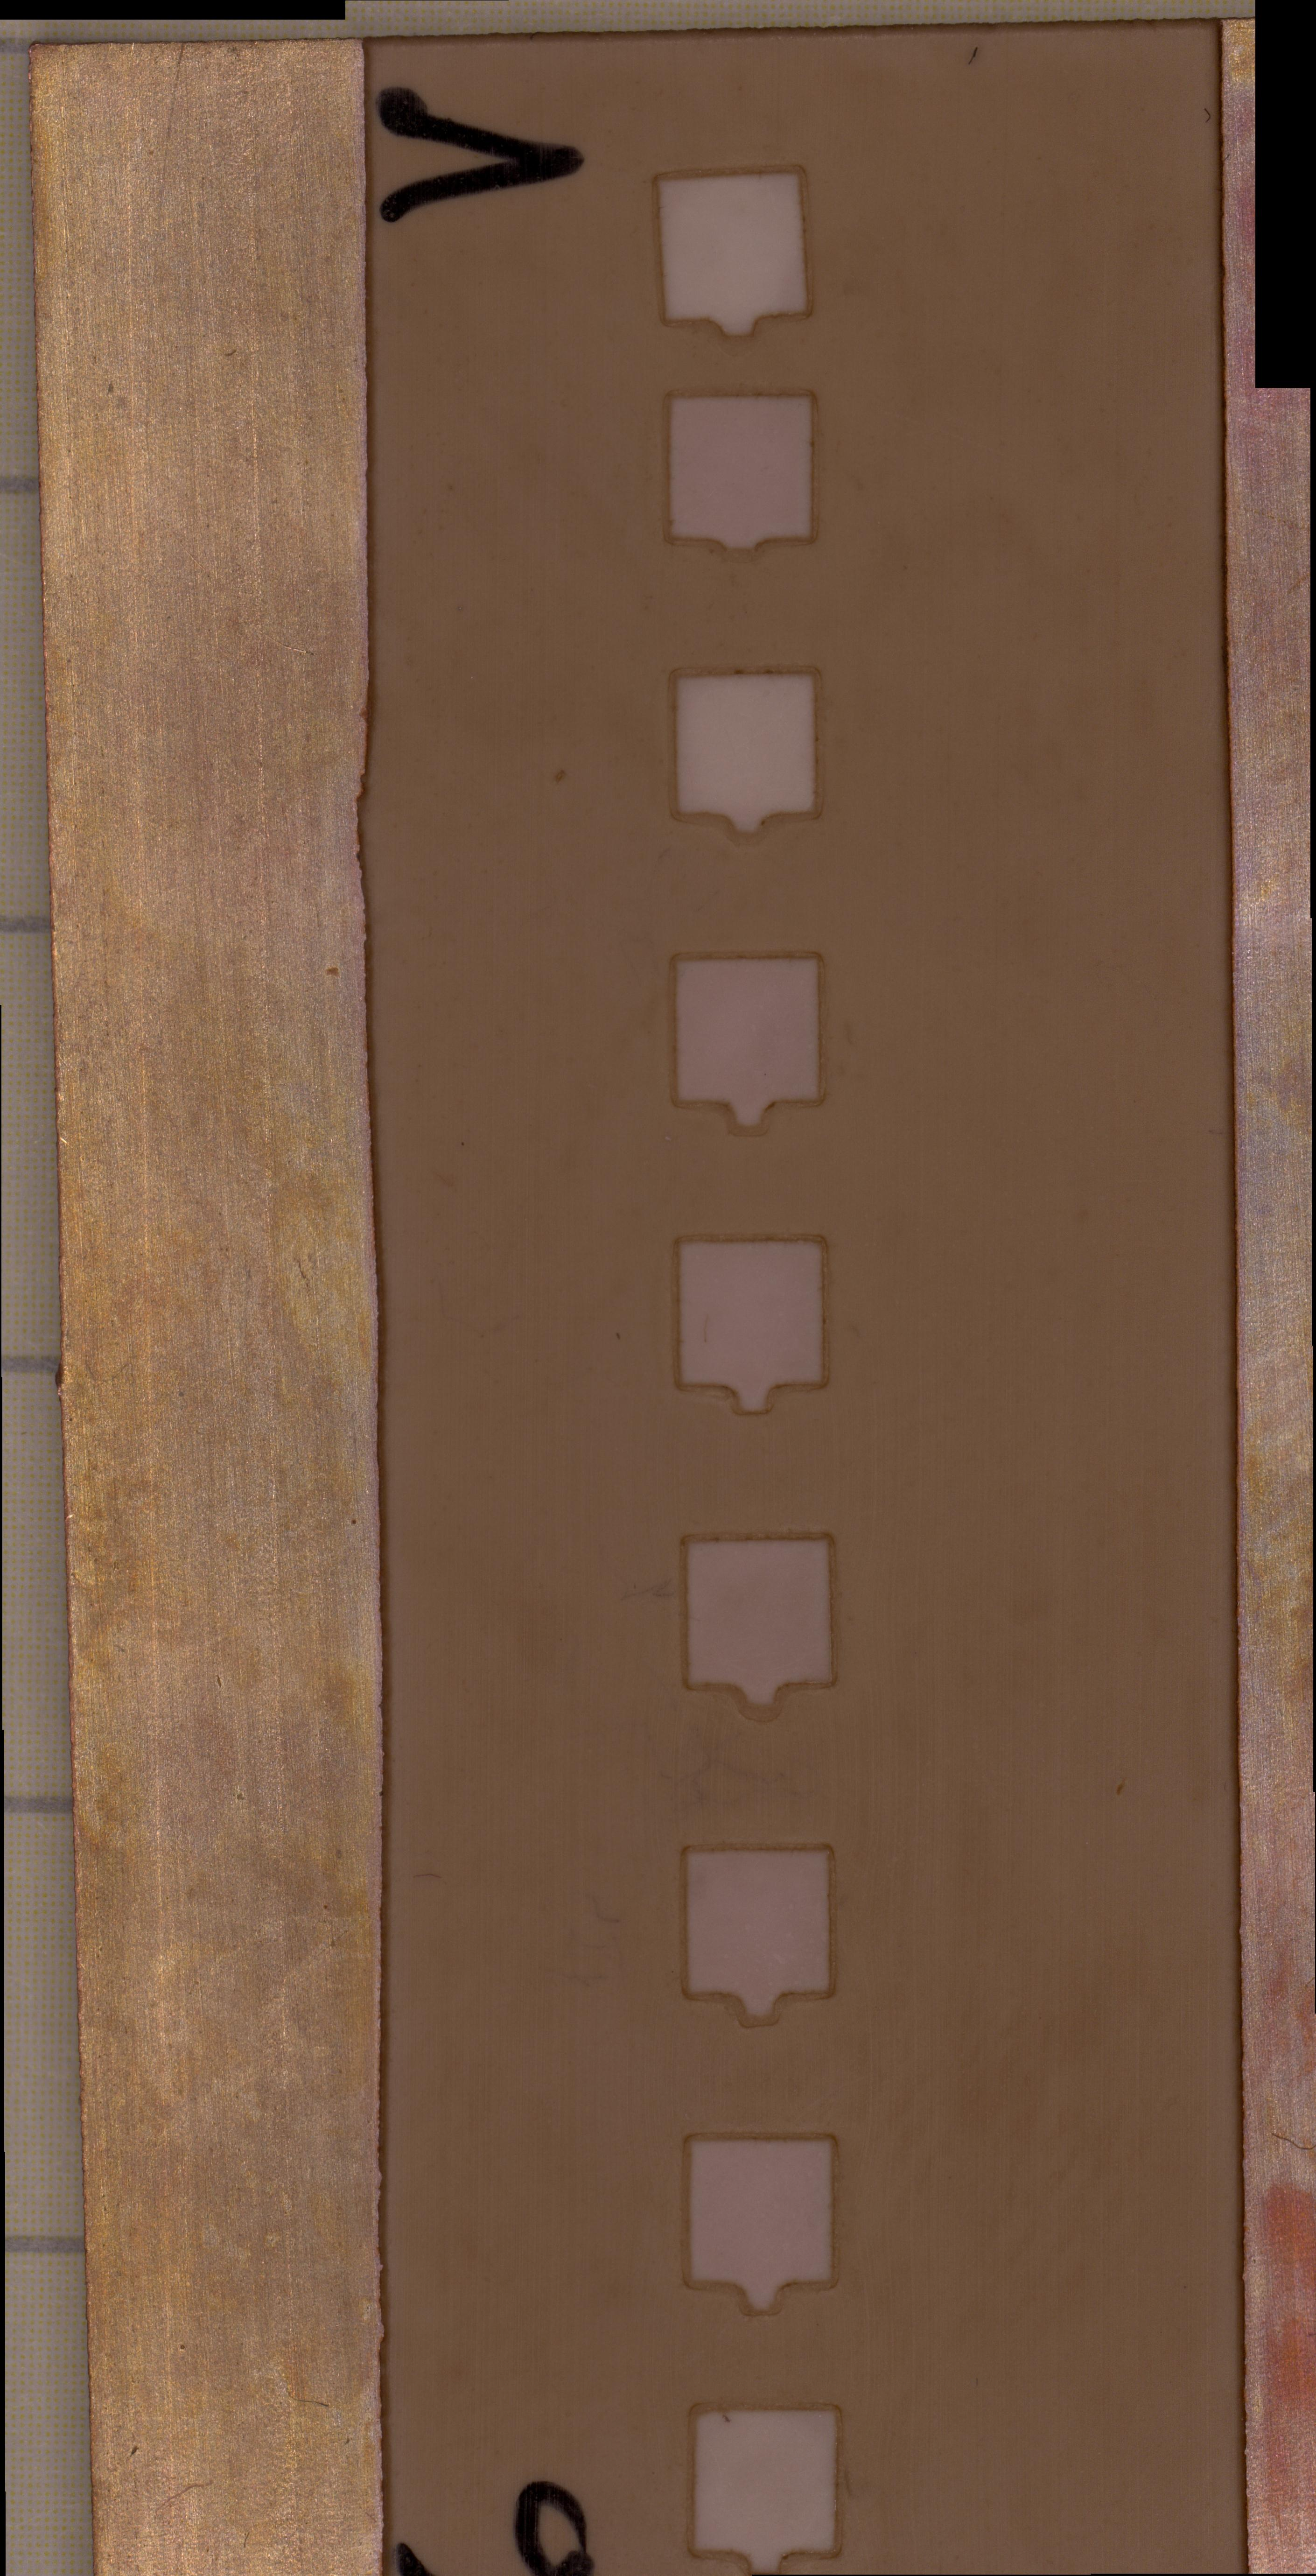
\includegraphics[scale=0.06, angle=90]{Bilder/Laminieren_Bodenplatte_Gesamt.jpg}
    \caption{Kupfer Scherkörper laminiert auf Kupferbodenplatte}
    \caption*{\textit{Quelle: Selbsterstellt}}
    \vspace{0.2cm}
    \label{Abb.3: Kupfer Scherkörper laminiert auf Kupferbodenplatte}
\end{figure}
\newpage
\subsection{Durchführung:}
Jeder Prüfling besitzt in seiner Platte zehn Scherkörper, die durch Schubspannung mit einem Schermeißel abgeschert werden.
\vspace{0.1cm}
\begin{figure}[h]
    \centering
    \includegraphics[scale=0.4]{Bilder/Schermeißel.png}
    \caption{Schertester Condor Sigma des Herstellers XYZTec}
    \caption*{\textit{Quelle: Selbsterstellt}}
    \vspace{0.2cm}
    \label{Abb.4: Schertester Condor Sigma des Herstellers XYZTec}
\end{figure}
\vspace{0.1cm}
Jeder der Prüfkörper wird nach dem Scheren auf eine Karteikarte geklebt, wobei der jeweilige Kraftwert eingetragen wird.
Dieser Wert wird aus der Computersoftware abgelesen.
\subsection{Untersuchung}
Nach Durchführung der Scherversuche werden die Bruchstellen der Prüfkörper mithilfe eines Digitalmikroskops untersucht und festgehalten.
Dabei steht die Identifizierung und Analyse der entstandenen Bruchmuster im Fokus. 

%------------------------------------------------------
%######################################################
%------------------------------------------------------

%\newpage
\section{Projektmanagement}
Der Laborversuch wurde am Freitag, den 21. März 2025, durchgeführt und innerhalb von 90 Minuten abgeschlossen.
\subsection{Einleitung und Vorbereitung}
Vor Beginn des Experiments fand eine kurze Einführung in das Thema Scherversuche statt. Dabei wurden die theoretischen Grundlagen erläutert, um das Verständnis für das Versuchsprinzip zu gewährleisten.
Im Anschluss erfolgte eine Anweisung zur Nutzung der Messgeräte, begleitet von einer Erklärung zu den verwendeten Messproben und den zu erwartenden Versuchsergebnissen.
Die Einweisung und Anweisung wurden von Prof. Dr.-Ing. Aylin Bicakci oder dem Laborpersonal durchgeführt.
\subsection{Meilsteine}
\begin{itemize}
    \item Verständnis der Messgeräte – Kennenlernen und richtige Handhabung der Geräte.
    \item Unterscheidung verschiedener Brucharten – Erkennen und Klassifizieren von Bruchmechanismen.
    \item Kritische Analyse – Bewertung der unterschiedlichen Bruchformen basierend auf Messwerten.
    \item Methodik der Scherversuche – Anwendung und Verinnerlichung des Prüfverfahrens.
    \item Erstellung des Laborberichts – Dokumentation der Ergebnisse und Analyse der Versuchsdaten.
\end{itemize}
\subsection{Struktur der Arbeit}
\subsection{Versuchsdurchführung}
Nach der theoretischen Einführung begann der Versuch. Während der Durchführung wurden die Messwerte sorgfältig beobachtet, gespeichert und dokumentiert.


%------------------------------------------------------
%######################################################
%------------------------------------------------------

\section{Proben und Methoden}
Der durchgeführte Schertest basiert auf der Norm MIL-STD-883E und untersuchte zwei verschiedene Scherprüflinge:
\begin{enumerate}
    \item Scherprüfling 1: Versilberte Kupferscherkörper, gesintert auf einer Kupferbodenplatte
    \item Scherprüfling 2: Kupferscherkörper, laminiert auf einer Kupferbodenplatte.
\end{enumerate}
Jeder Scherkörper bestand aus acht Scherprüflingen, die mithilfe eines Klebstoffs auf der Kupferbodenplatte fixiert wurden.
Für den Schertest wurden folgende Prüfgeräte verwendet:
\begin{itemize}
    \item Schertester Condor Sigma der Firma XYZTec
    \item Digitalmikroskop zur hochauflösenden Analyse der Bruchflächen
\end{itemize}
Für dieses Schertest ist sowohl ein Schertester Condor Sigma von der Firma XYZTec als auch ein Digitalmikroskop  zu nutzen. 
\subsection{Schertester Condor Sigma von XYZTec}
Der Schertester besteht aus einem Schermeißels, ein Mikroskop und sein eigener Rechner. 
Der XYZTec Condor Sigma ist ein hochmoderner Schertester, der für präzise und automatisierte Prüfungen von Verbindungen in der Halbleiter und Elekronikindustrie entwickelt wurde:
Der Schetester besitzt die folgende Eigenschaften:
\begin{itemize}
    \item Modularer Aufbau: Der Condor Sigma verfügt über eine modulare Architektur, die es ermöglicht, verschiedene Testköpfe zu integrieren, darunter die Rotierende Messeinheit RMU mit bis zu sechs Sensoren. Dies erlaubt kontinuierliche Tests ohne manuelle Umrüstungen. 
    \item Automatisierung: Das System bietet umfassende Automatisierungsfunktionen, einschließlich roboterbasierter Handhabung für sicheres Laden und Entladen von Proben. Die offene Sigma-Software ermöglicht eine einfache Programmierung aller Automatisierungsschritte mithilfe von Kameravisualisierung und intelligenten Assistenten.
    \item Präzise Positionskontrolle: Ein integrierter dynamischer Motion-Controller und lineare Encoder verbessern die Positionsgenauigkeit und Reproduzierbarkeit in den X-, Y- und Z-Achsen erheblich.
    \item Hohe Messgenauigkeit: Der Nano-Control-Scherkraftsensor ermöglicht eine außergewöhnliche Präzision in der Scherhöhenmessung mit einer Genauigkeit von bis zu 200 nm. 
    \item Vielseitige Testmöglichkeiten: Der Condor Sigma kann für verschiedene Testarten wie Scher-, Zug- und Drucktests konfiguriert werden und deckt dabei einen Kraftbereich von weniger als 0,1 gf bis zu 10 kgf ab. 
    \item Hochauflösende Bildgebung: Das System unterstützt bis zu drei Live-Kameras mit flexibler LED-Beleuchtung und bietet umfangreiche Bildverarbeitungsoptionen für detaillierte optische Inspektionen. cite{2}
\end{itemize}
\subsubsection{Vorteile von dem XYZTec Condor Sigma}
\begin{enumerate}
    \item Flexibilität: Dank des modularen Designs kann der Condor Sigma an spezifische Prüfanforderungen angepasst werden, was eine hohe Vielseitigkeit in verschiedenen Anwendungen ermöglicht.
    \item Effizienzsteigerung: Die umfassende Automatisierung reduziert menschliche Fehler und senkt Produktionskosten durch schnellere und konsistentere Prüfprozesse.
    \item Benutzerfreundlichkeit: Die intuitive Softwareoberfläche und die einfache Programmierung erleichtern die Bedienung und verkürzen die Einarbeitungszeit für das Personal.
    \item Zukunftssicherheit: Durch kontinuierliche Verbesserungen und Updates bleibt der Condor Sigma auf dem neuesten Stand der Technik und erfüllt aktuelle sowie zukünftige Prüfanforderungen.cite{3}
\end{enumerate}
\subsection{Einsatz des Digitalmikroskops}
Während des Versuchs wurde ein hochauflösendes Digitalmikroskop verwendet, um die Bruchflächen detailliert zu analysieren. Dies ermöglichte eine präzise Auswertung der Bruchmechanismen und eine zuverlässige Beurteilung der Materialeigenschaften.


%------------------------------------------------------
%######################################################
%------------------------------------------------------

\section{Durchführung}
\input{Sections/06-Durchführung}


%------------------------------------------------------
%######################################################
%------------------------------------------------------

\section{Ergebnisse}
\subsection{Sintern.....}

\begin{table}[H]
\centering

\adjustbox{max width=\textwidth}{

% Resize the table to fit within the page
%\resizebox{\textwidth}{!}{%


\renewcommand{\arraystretch}{1.7} % Increase row height (local)
\fontsize{18pt}{20pt}\selectfont
\begin{tabular}{|l|c|c|c|c|}
\hline
\textbf{Scherkörper} & \multicolumn{1}{l|}{\textbf{Maximale Scherkraft} {[}\si{\newton}{]}} & \multicolumn{1}{l|}{\textbf{Durchschnittskraft} {[}\si{\newton}{]}} & \multicolumn{1}{l|}{\textbf{Fläche} {[}\si{\milli\meter\squared}{]}} & \multicolumn{1}{l|}{\textbf{Scherfestigkeit} {[}\si{\newton\per\milli\meter\squared}{]}} \\ \hline
\textbf{1} & 330,45 & 143,11 & 5,29 & 62,47 \\ \hline
\textbf{2} & 459,23 & 137,78 & 5,29 & 86,81 \\ \hline
\textbf{3} & 420,47 & 135,23 & 5,29 & 79,48 \\ \hline
\textbf{4} & 384,35 & 148,57 & 5,29 & 72,66 \\ \hline
\textbf{5} & 508,97 & 172,81 & 5,29 & 96,21 \\ \hline
\textbf{6} & 358,84 & 116,34 & 5,29 & 67,83 \\ \hline
\textbf{7} & 388,41 & 143,01 & 5,29 & 73,42 \\ \hline
\textbf{8} & 354,98 & 140,97 & 5,29 & 67,10 \\ \hline
\end{tabular}}
\vspace{0.5cm}
\caption{Sintern}
\label{Tab.1}
\end{table}




\begin{table}[H]
\centering

\adjustbox{max width=\textwidth}{

% Resize the table to fit within the page
%\resizebox{\textwidth}{!}{%


\renewcommand{\arraystretch}{1.7} % Increase row height (local)
\fontsize{18pt}{20pt}\selectfont
\begin{tabular}{|l|c|c|c|c|}
\hline
\textbf{Scherkörper} & \multicolumn{1}{l|}{\textbf{Maximale Scherkraft} {[}\si{\newton}{]}} & \multicolumn{1}{l|}{\textbf{Durchschnittskraft} {[}\si{\newton}{]}} & \multicolumn{1}{l|}{\textbf{Fläche} {[}\si{\milli\meter\squared}{]}} & \multicolumn{1}{l|}{\textbf{Scherfestigkeit} {[}\si{\newton\per\milli\meter\squared}{]}} \\ \hline
\textbf{1} & 195,05 & 77,34 & 5,29 & 36,87 \\ \hline
\textbf{2} & 146,72 & 55,16 & 5,29 & 27,74 \\ \hline
\textbf{3} & 143,32 & 47,98 & 5,29 & 27,09 \\ \hline
\textbf{4} & 129,39 & 39,87 & 5,29 & 24,46 \\ \hline
\textbf{5} & 142,67 & 54,48 & 5,29 & 26,97 \\ \hline
\textbf{6} & 128,16 & 51,59 & 5,29 & 24,23 \\ \hline
\textbf{7} & 147,18 & 70,87 & 5,29 & 27,82 \\ \hline
\textbf{8} & 131,37 & 49,35 & 5,29 & 24,83 \\ \hline
\textbf{9} & 175,58 & 78,33 & 5,29 & 33,19 \\ \hline
\end{tabular}}
\vspace{0.5cm}
\caption{Laminiert}
\label{Tab.2}
\end{table}





\begin{tikzpicture}
	% Read the data from the CSV
	\pgfplotstableread[col sep=comma]{data.csv}\csvdata
	
	% Transpose the data (rows become columns)
	\pgfplotstabletranspose\datatransposed{\csvdata} 
	
	\begin{axis}[
		boxplot/draw direction = y,    % Draw boxplot in horizontal direction
		x axis line style = {opacity=0},
		axis x line* = bottom,
		axis y line = left,
		enlarge y limits,
		ymajorgrids,
		xtick = {1, 2},               % Define x-ticks
		xticklabel style = {align=center, font=\small, rotate=60},
		xticklabels = {Sintern, Laminiert},
		xtick style = {draw=none},     % Hide tick lines
		ylabel = {Scherfestigkeit \si{\newton\per\milli\meter\squared}}, % Y-axis label
	]
		% Plot the boxplots for each dataset (column in the transposed data)
		\foreach \n in {1, 2} {  % Only 2 columns after transpose
			\addplot+[boxplot, fill, draw=black] table[y index=\n] {\datatransposed};
		}
	\end{axis}
\end{tikzpicture}



%------------------------------------------------------
%######################################################
%------------------------------------------------------

\section{Zusammenfassung}
Die durchgeführten Schertests verdeutlichen den erheblichen Einfluss der Materialwahl auf die mechanischen Eigenschaften der Prüfkörper. Gesinterte Scherkörper zeigen konsistent höhere Scherfestigkeiten und stabilere Bruchmechanismen im Vergleich zu laminierten Proben, was darauf hinweist, dass das Sintern eine festere und langlebigere Verbindung erzeugt als die Laminierung.\\

Es ist jedoch zu berücksichtigen, dass die Prüfkörper manuell auf die Bodenplatte aufgesetzt wurden, was potenziell Einfluss auf die Messergebnisse hatte. Diese manuelle Platzierung könnte zu Variationen in der Ausrichtung oder der Kontaktfläche geführt haben und somit die Messergebnisse beeinflusst haben. Eine standardisierte, automatisierte Positionierung könnte die Reproduzierbarkeit und Genauigkeit zukünftiger Untersuchungen weiter verbessern.\\

Die gewonnenen Messergebnisse liefern eine wertvolle Grundlage für industrielle Anwendungen, insbesondere in Bereichen mit hohen mechanischen Belastungen. Die Analyse der Bruchbilder bestätigt zudem die theoretischen Annahmen über die Bruchmechanismen der jeweiligen Herstellungsverfahren und bietet weiterführende Erkenntnisse für die Optimierung der Materialauswahl und Fertigungsprozesse.

%------------------------------------------------------
%######################################################
%------------------------------------------------------

\section{Fazit}
Der durchgeführte Schertest analysiert die mechanischen Eigenschaften gesinterter und laminierter Kupferscherkörper gemäß der Norm MIL-STD-883E. Die Versuchsdurchführung erfolgte mithilfe eines Schertesters sowie eines hochauflösenden Digitalmikroskops zur detaillierten Untersuchung der Bruchbilder. Ziel der Studie war die Bestimmung der maximalen und durchschnittlichen Scherkraft sowie der Scherfestigkeit der Prüfkörper, um die Unterschiede zwischen beiden Herstellungsverfahren systematisch herauszuarbeiten. Darüber hinaus diente der Versuch zur Evaluierung des Schertests, der verwendeten Messgeräte und des experimentellen Laborumfelds.\\

Neben der Bestimmung der Scherfestigkeit wurde die Streuung der Messergebnisse analysiert. Die individuellen Abweichungen der Prüfkörper wurden statistisch ausgewertet und in einem Boxplot visualisiert, um eine differenzierte Beurteilung der Messwerte und ihrer Variabilität zu ermöglichen.\\

Die Untersuchungsergebnisse zeigen signifikante Unterschiede zwischen gesinterten und laminierten Prüfkörpern. Gesinterte Scherkörper weisen eine höhere maximale Scherkraft und Scherfestigkeit auf, was auf eine festere und belastbarere Verbindung zwischen Scherkörper und Bodenplatte hindeutet. Die Bruchbildanalyse bestätigt diese Beobachtung durch charakteristische Unterschiede in den Bruchmechanismen.
\newpage

%------------------------------------------------------
%######################################################
%------------------------------------------------------

%\section{Formelzeichen}
%\input{Sections-ending/09-Formelzeichen}

%------------------------------------------------------
%######################################################
%------------------------------------------------------



%------------------------------------------------------
%######################################################
%------------------------------------------------------
\newpage
\section{Abbildungsverzeichnis}
\listoffigures

%------------------------------------------------------
%######################################################
%------------------------------------------------------

\section{Tabellenverzeichnis}
\listoftables

%------------------------------------------------------
%######################################################
%------------------------------------------------------

\section{Literaturverzeichnis}
\printbibliography
%\input{Aufgaben/05-Literaturverzeichnis}
%\printbibliography
%------------------------------------------------------
%######################################################
%------------------------------------------------------

%------------------------------------------------------
%######################################################
%------------------------------------------------------


%------------------------------------------------------
%--------------------Vorlage-Testing-------------------
%------------------------------------------------------

%\section{Vorlage-Testing}
%\input{Vorlage/Figuren-Struktur}
%\input{Vorlage/Tabellen-Struktur}


\newpage

\end{document}
